\documentclass[11pt]{article}
\usepackage[margin=1in]{geometry}
\usepackage{amsmath,amssymb}
\usepackage{booktabs}
\usepackage{graphicx}
\usepackage{hyperref}
\usepackage[T1]{fontenc}
\newcommand{\code}[1]{\texttt{#1}}
\title{The Bounded Curated Store vs.\ the Regular-Only Regime:\\
Contract, Selection Rule, and the 2026-07-30/31 Measurement Campaign}
\author{local\_mixing working notes}
\date{2026-07-31}

\begin{document}
\maketitle

\begin{abstract}
The new bounded curated \code{.frz} store (1.72\,GB; $\le$20 candidates and
$\le$512 decoded value bytes per key) was installed, its runtime contract
implemented (per-store value conventions, expansion-first routing), and a
two-scale measurement campaign run against the regular-only baselines: 15
arms on the 20k-gate/64-wire sample and 6 arms on the 100k-gate/512-wire
slices, all same-seed pairs. Headline: the curated cascade wins on every
measured axis at every scale --- circuits up to 71\% smaller, ancestry
transport up to $+149\%$, schedule and slice asymmetries largely erased ---
with \textbf{zero} verification rejections across $\sim$2M curated splices.
The splice-economy decomposition shows why: curated conversions are a
dedicated growth stroke (58--62\% growing, $+2$-dominated), non-curated
conversions a dedicated compression stroke ($\sim$24\% shrinking,
$\sim$0\% growing) --- two stores, each doing the job it is built for. A
$2{\times}2$ interaction check shows the conclusion is robust to (and
strengthened by) turning on \code{--db-advance}, which was off throughout
the campaign.
\end{abstract}

\section{The stores}

\textbf{Old (retired):} the unbounded curated store --- 6.49\,GB, 258
files, a pathological 1.19\,GB \code{shard\_66} --- kept at
\code{frozen\_curated\_m1\_m11.old6g}. Every historical ``430k candidates /
multi-megabyte values / never reaches its first checkpoint'' observation
describes this store.

\textbf{New (installed, verified):} \code{/home/cc/frozen\_curated\_m1\_m11},
1{,}720{,}215{,}364 bytes; \code{shard\_66.frz} $= 6{,}350{,}369$ B;
\code{tables.bin} \code{df8ee453\ldots}; \code{filters.bin}
\code{8dde6635\ldots}. Bounded guarantees: $\le$20 candidates/key, $\le$512
decoded value bytes/key, largest encoded bucket 361\,B. Reference lookup
cost: 3.8\,$\mu$s curated, 33\,$\mu$s regular.

\textbf{The convention fix.} The curated store was built under the
pre-\code{2ed0222a} swapped-controls polynomial key convention, so its
values decode with each gate's two controls swapped relative to native ---
the never-diagnosed root cause of ``every curated candidate fails
verification.'' The runtime now takes per-store conventions from the
environment (\code{FROZEN\_REGULAR\_VALUE\_CONVENTION=native},
\code{FROZEN\_CURATED\_VALUE\_CONVENTION=legacy-swapped-controls}),
applying a controls-swap at the single decode choke point. Proof at scale:
\code{cur=hits/0} --- zero rejections --- in every run of the campaign,
under mandatory per-splice exhaustive verification.

\section{Routing and selection}

Commits \code{f8afdc7b} + \code{47053b0f}:

\begin{itemize}
\item \textbf{Expansion (MIX / ANY)}: probe CURATED first, forward key
only. Apply the mode's size rule within the curated answer --- for MIX:
\emph{random among no-larger spellings if any exist, else random among the
minimal ones}. On a complete curated miss, fall back to REGULAR (forward +
reverse keys) under the same rule. The reverse canonicalization is deferred
to the fallback stage.
\item \textbf{Compression}: REGULAR only, always --- including the ssg
SAMF-hiding tiers.
\item Tripwire: a warn-once alarm if any curated value exceeds the bounded
contract.
\end{itemize}

\section{Campaign design}

Same-seed pairs, only the store policy changed. \textbf{20k battery:} the
A/B/C schedule family (A phased 200k MIX $\to$ COMP; B \code{p\_mix} 0.2; C
0.1) $\times$ \{no twist, legacy twists 0.002/0.01, g57-v2 twists
0.002/0.01\}, 2M moves, exact ancestry. \textbf{100k battery:} slices 1
and 2 of the $n{=}128$ Gray gadget (512 wires) $\times$ \code{p\_mix}
\{0.20, 0.10, 0.05\}, 2.877M moves, sampled ancestry ($K{=}256$).
\code{--db-advance} was off throughout (both columns --- internally
consistent; \S6 measures the flag's effect). \code{FROZEN\_FILTER} off for
the battery (trajectory-identical; filters only accelerate misses).

\section{Results}

\subsection{20k sample}

\begin{table}[h]\centering\small
\begin{tabular}{lrrrr}
\toprule
arm & size old$\to$new & anc old$\to$new & span old$\to$new & eff old$\to$new \\
\midrule
A no twist & 64{,}333 $\to$ \textbf{24{,}320} & 2{,}649 $\to$ \textbf{6{,}606} & 3{,}253 $\to$ 7{,}112 & 24.9 $\to$ 61.7 \\
A legacy .002 & 135{,}058 $\to$ 90{,}770 & 187 $\to$ 164 & 691 $\to$ 577 & 16.2 $\to$ 20.3 \\
A legacy .01 & 247{,}382 $\to$ 227{,}632 & 69 $\to$ 64 & 393 $\to$ 327 & 12.5 $\to$ 12.9 \\
A g57v2 .002 & 107{,}220 $\to$ \textbf{54{,}678} & 1{,}085 $\to$ \textbf{1{,}673} & 1{,}690 $\to$ 2{,}121 & 19.7 $\to$ 35.9 \\
A g57v2 .01 & 202{,}164 $\to$ 142{,}886 & 447 $\to$ 441 & 973 $\to$ 890 & 14.1 $\to$ 18.5 \\
B no twist & 121{,}835 $\to$ \textbf{35{,}213} & 3{,}165 $\to$ \textbf{7{,}527} & 3{,}820 $\to$ 8{,}159 & 32.9 $\to$ 60.2 \\
B legacy .002 & 243{,}674 $\to$ 211{,}770 & 350 $\to$ 350 & 1{,}012 $\to$ 954 & 21.5 $\to$ 23.0 \\
B legacy .01 & 383{,}924 $\to$ 373{,}367 & 80 $\to$ 90 & 451 $\to$ 443 & 16.2 $\to$ 16.4 \\
B g57v2 .002 & 157{,}153 $\to$ \textbf{72{,}929} & 1{,}895 $\to$ \textbf{2{,}602} & 2{,}589 $\to$ 3{,}275 & 28.0 $\to$ 40.0 \\
B g57v2 .01 & 270{,}377 $\to$ 175{,}873 & 620 $\to$ 825 & 1{,}198 $\to$ 1{,}410 & 19.7 $\to$ 23.5 \\
C no twist & 48{,}493 $\to$ 25{,}804 & 7{,}941 $\to$ \textbf{9{,}615} & 8{,}626 $\to$ 10{,}340 & 55.5 $\to$ 76.0 \\
C legacy .002 & 133{,}665 $\to$ 120{,}777 & 425 $\to$ 479 & 1{,}111 $\to$ 1{,}211 & 31.8 $\to$ 33.6 \\
C legacy .01 & 262{,}115 $\to$ 259{,}558 & 62 $\to$ 71 & 369 $\to$ 399 & 21.4 $\to$ 21.3 \\
C g57v2 .002 & 78{,}233 $\to$ \textbf{54{,}031} & 3{,}038 $\to$ 3{,}339 & 3{,}895 $\to$ 4{,}098 & 42.0 $\to$ 50.6 \\
C g57v2 .01 & 168{,}192 $\to$ 132{,}681 & 921 $\to$ 1{,}012 & 1{,}625 $\to$ 1{,}661 & 26.1 $\to$ 28.8 \\
\bottomrule
\end{tabular}
\caption{Finals at 2M moves. Sizes fall everywhere (most where MIX
dominates); transport rises with effective work; the A/B/C schedule gap
largely collapses (all no-twist baselines land at 24--35k gates, eff
60--76). All prior orderings (twist arms, rates) survive.}
\end{table}

\subsection{100k / 512-wire slices}

\begin{table}[h]\centering\small
\begin{tabular}{lrrrr}
\toprule
run & size old$\to$new & est.\ anc old$\to$new & cov old$\to$new & ent old$\to$new \\
\midrule
s1 \code{p\_mix}.20 & 275{,}431 $\to$ \textbf{183{,}160} & 12{,}591 $\to$ \textbf{19{,}273} & .183 $\to$ \textbf{.245} & .518 $\to$ .612 \\
s2 \code{p\_mix}.20 & 284{,}635 $\to$ \textbf{177{,}101} & 17{,}901 $\to$ 21{,}330 & .254 $\to$ .266 & .606 $\to$ .635 \\
s1 \code{p\_mix}.10 & 178{,}592 $\to$ \textbf{142{,}212} & 22{,}774 $\to$ \textbf{27{,}678} & .298 $\to$ \textbf{.339} & .651 $\to$ .692 \\
s2 \code{p\_mix}.10 & 179{,}136 $\to$ 137{,}094 & 29{,}009 $\to$ 30{,}360 & .363 $\to$ .369 & .709 $\to$ .719 \\
s1 \code{p\_mix}.05 & 136{,}927 $\to$ 125{,}059 & 30{,}031 $\to$ 31{,}562 & .383 $\to$ .389 & .711 $\to$ .720 \\
s2 \code{p\_mix}.05 & 135{,}334 $\to$ 120{,}482 & 33{,}443 $\to$ 33{,}658 & .416 $\to$ .743$^{\approx}$ & $\approx$ \\
\bottomrule
\end{tabular}
\caption{Production scale replicates the 20k findings; gains scale with the
MIX fraction. The old slice-1-vs-slice-2 asymmetry (12.6k vs.\ 17.9k anc at
\code{p\_mix} .20) closes under the cascade (19.3k vs.\ 21.3k).}
\end{table}

\subsection{Dynamics}

\textbf{Curated share of successful splices} is flat over each 20k run
(C $\approx$ 0.17, B $\approx$ 0.28; legacy arms higher via a weak-COMP
denominator) and, on the 100k slices, decays from an early store-friendly
peak to stable plateaus ($\approx$ .08/.15/.26 by \code{p\_mix}) --- the
store keeps serving at the same rate deep into the run, and slice-1/slice-2
curves are near-identical.

\textbf{Grow/shrink balance}: the cascade lowers the growing-conversion
fraction by 1--6 points and raises the shrinking fraction (B no-twist
cumulative $0.147 \to 0.200$), which no longer decays late-run --- COMP
stays productive against the smaller steady-state circuit.

\subsection{The splice-economy decomposition}

A per-store splice histogram (instrumented rerun; bit-identical
trajectories verified at both scales) splits the successful-splice
$(\mathrm{out} \to \mathrm{in})$ distribution:

\begin{table}[h]\centering\small
\begin{tabular}{lrrrrl}
\toprule
population & n & shrink & equal & grow & shape \\
\midrule
(a) old regular-only (20k B) & 710k & .147 & .690 & .164 & grow spread $+2/+3/+4$ \\
(b) new total (20k B) & 809k & .200 & .641 & .160 & grow at $+2$ and $+6$ \\
(c) new, curated only & 220k & .087 & .334 & \textbf{.579} & $+2$ (30\%), $+6$ (20\%) \\
(d) new, non-curated & 589k & \textbf{.242} & .756 & .003 & $-2/-4/-6$ only \\
\midrule
100k: curated only & 601k & .079 & .305 & .616 & same shape \\
100k: non-curated & 1.62M & .233 & .760 & .007 & same shape \\
\bottomrule
\end{tabular}
\caption{The two-stroke engine: curated conversions are the growth stroke
(the store holds longer equivalents by construction --- splits of minimal
identities --- so the ``else random minimal'' branch dominates, usually at
$+2$), non-curated conversions the compression stroke ($\sim$zero growth).
The old regime forced one store to do both jobs.}
\end{table}

\section{Robustness to \code{--db-advance}}

The whole campaign ran with \code{--db-advance} off (both columns). A
$2{\times}2$ same-seed interaction check at the strongest-effect point
(20k, C schedule, no twists) asks whether the flag changes the conclusion:

\begin{center}\small
\begin{tabular}{lrrrr}
\toprule
cell & size & anc & span & eff \\
\midrule
regular, off & 48{,}493 & 7{,}941 & 8{,}626 & 55.5 \\
curated, off & 25{,}804 & 9{,}615 & 10{,}340 & 76.0 \\
regular, on & 66{,}957 & 11{,}950 & 12{,}679 & 39.9 \\
curated, on & \textbf{27{,}761} & \textbf{15{,}637} & \textbf{16{,}305} & 60.6 \\
\bottomrule
\end{tabular}
\end{center}

The curated-vs-regular delta \emph{widens} with the flag on (anc $+1{,}674
\to +3{,}686$; size $-22.7$k $\to -39.2$k): ballistic transport amplifies
whichever splice economy is in place, and the curated economy is better
(the regular regime's growth-heavy splices both spread and accumulate).
The flag itself adds $+50$--$63\%$ transport in both regimes ---
\textbf{directive: \code{--db-advance} on in every run unless an A/B
explicitly needs it off}. The weak-effect bracket (100k slice-1,
\code{p\_mix} .05, both advance-on cells) was still running at the time of
writing; with the margin above, only a sign reversal there could matter.

\section{Conclusions}

\begin{enumerate}
\item The bounded curated store is correct (zero rejections at two scales
under exhaustive verification), fast (its lookups are not a cost factor),
and strictly beneficial under the cascade selection rule at every measured
operating point.
\item The mechanism is a division of labor: curated supplies re-encoding
diversity (growth in small, structured steps), regular supplies
compression. Routing each job to its store beats any single-store policy
measured.
\item The best measured operating point on the 20k sample is
\emph{curated + db-advance}: anc 15{,}637 at 27.8k gates --- $2\times$ the
transport of the best regular-only cell at half its size.
\item Caveats: campaign comparisons are same-seed single trajectories (no
replication); \code{--db-advance} was off in the battery (both sides;
\S5 shows on-state widens the win); campaign-preflight fingerprints still
pin the old store and need regeneration.
\end{enumerate}

\clearpage
\appendix
\section{Figures}

\begin{figure}[h]\centering
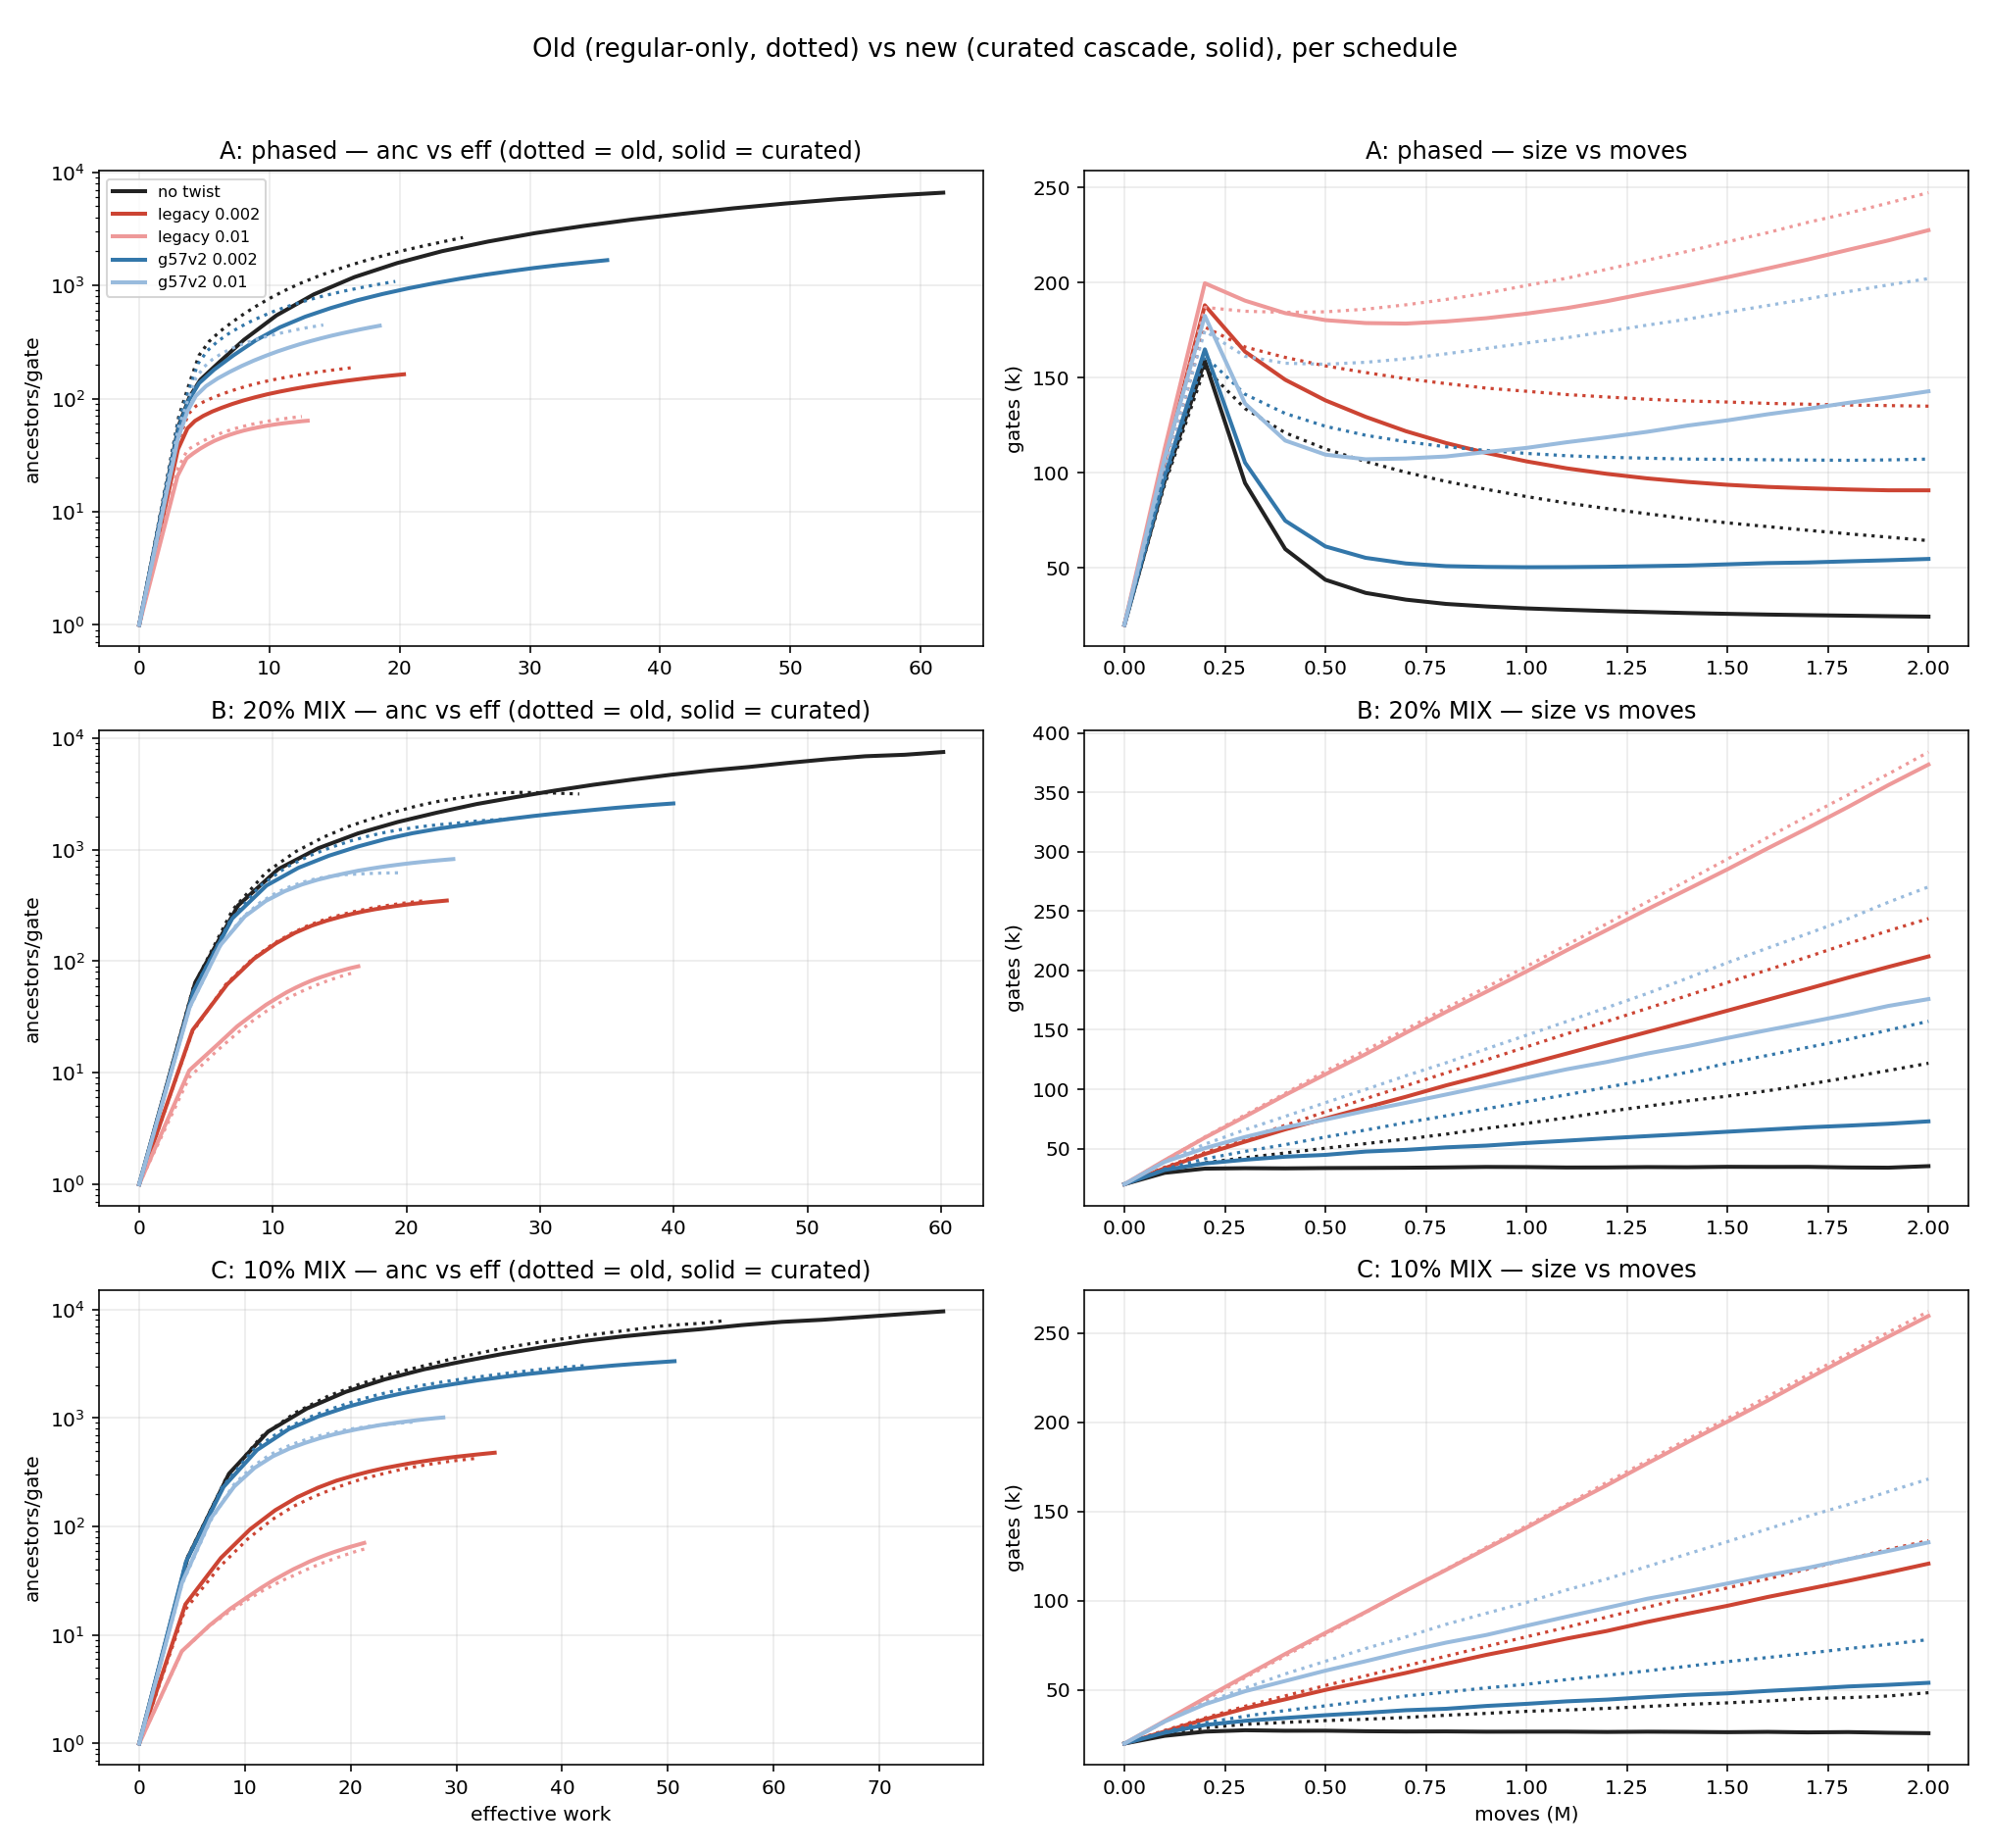
\includegraphics[width=\textwidth]{../reports/ancestry_20260728/abc_old_vs_curated_20260730.png}
\caption{Per-schedule overlays: old (dotted) vs.\ curated cascade (solid).}
\end{figure}
\begin{figure}[h]\centering
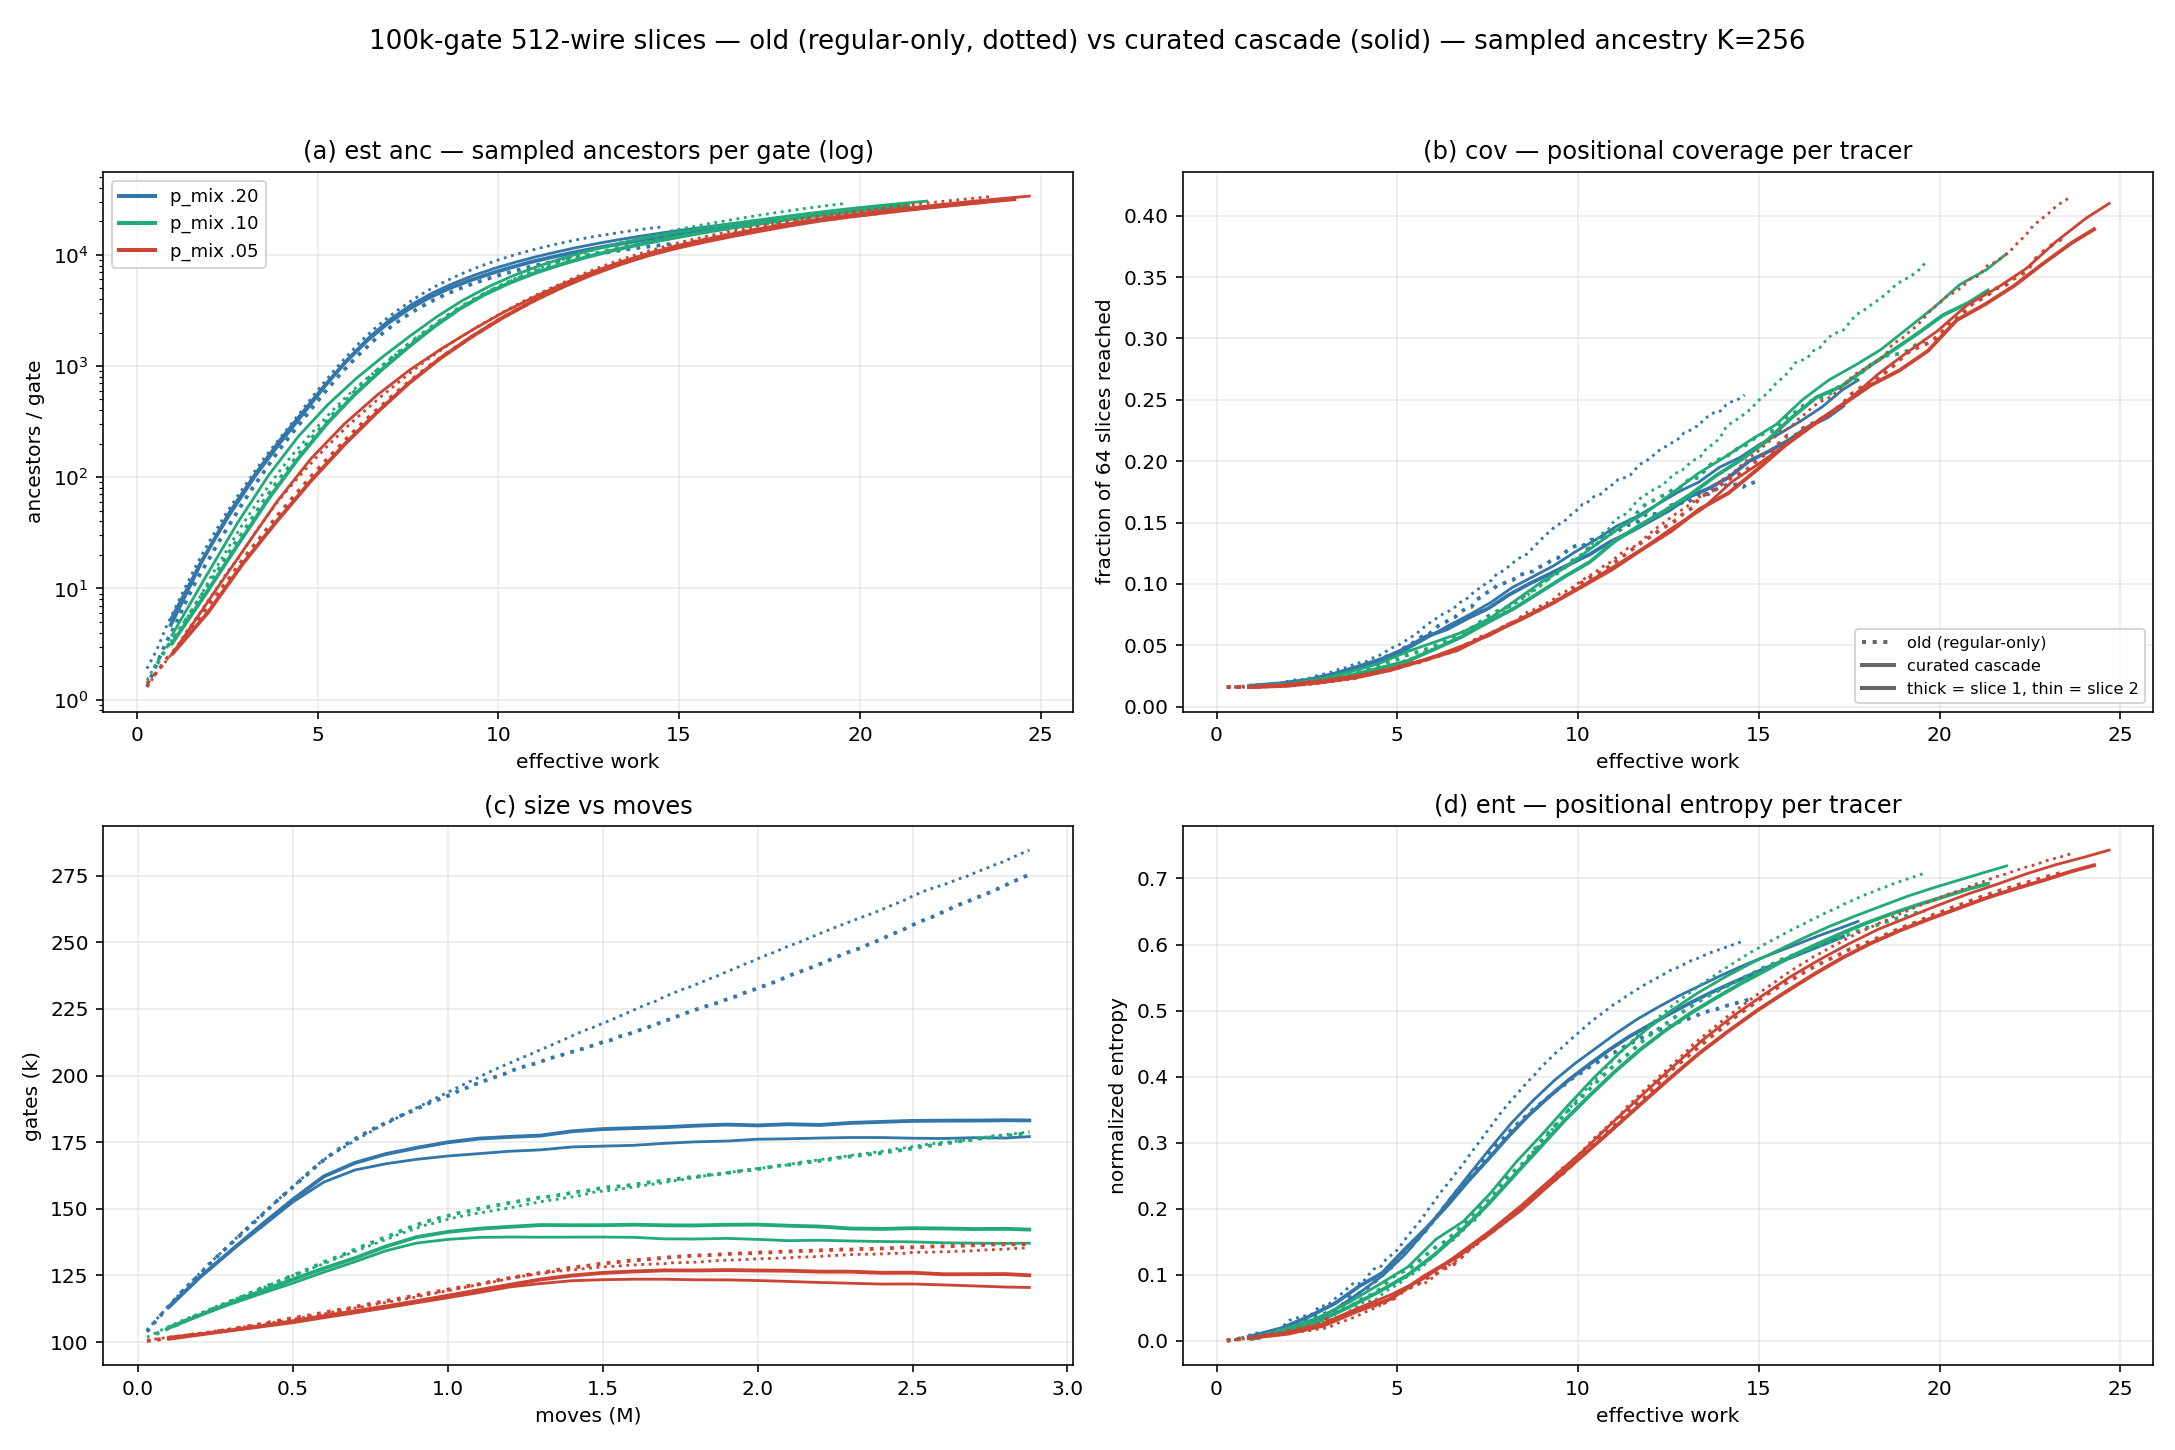
\includegraphics[width=\textwidth]{../reports/ancestry_20260728/bigslice_curated_20260730.png}
\caption{100k/512-wire slices: sampled-ancestry measures, old vs.\ new.}
\end{figure}
\begin{figure}[h]\centering
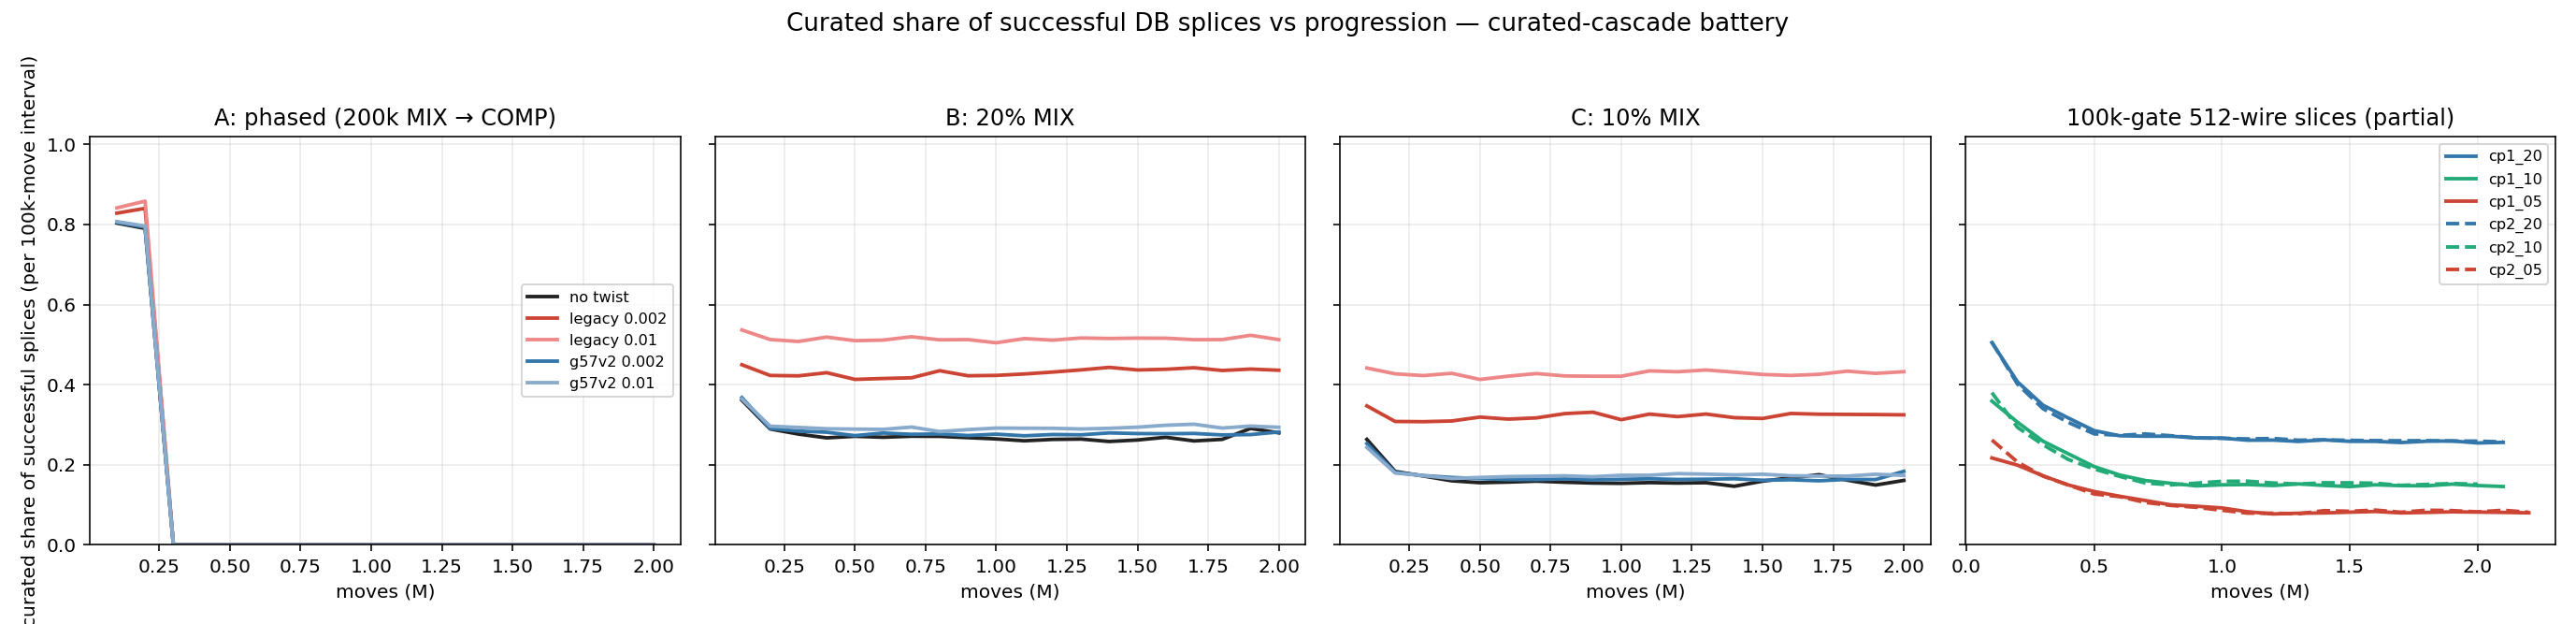
\includegraphics[width=\textwidth]{../reports/ancestry_20260728/curated_share_20260730.png}
\caption{Curated share of successful splices vs.\ progression.}
\end{figure}
\begin{figure}[h]\centering
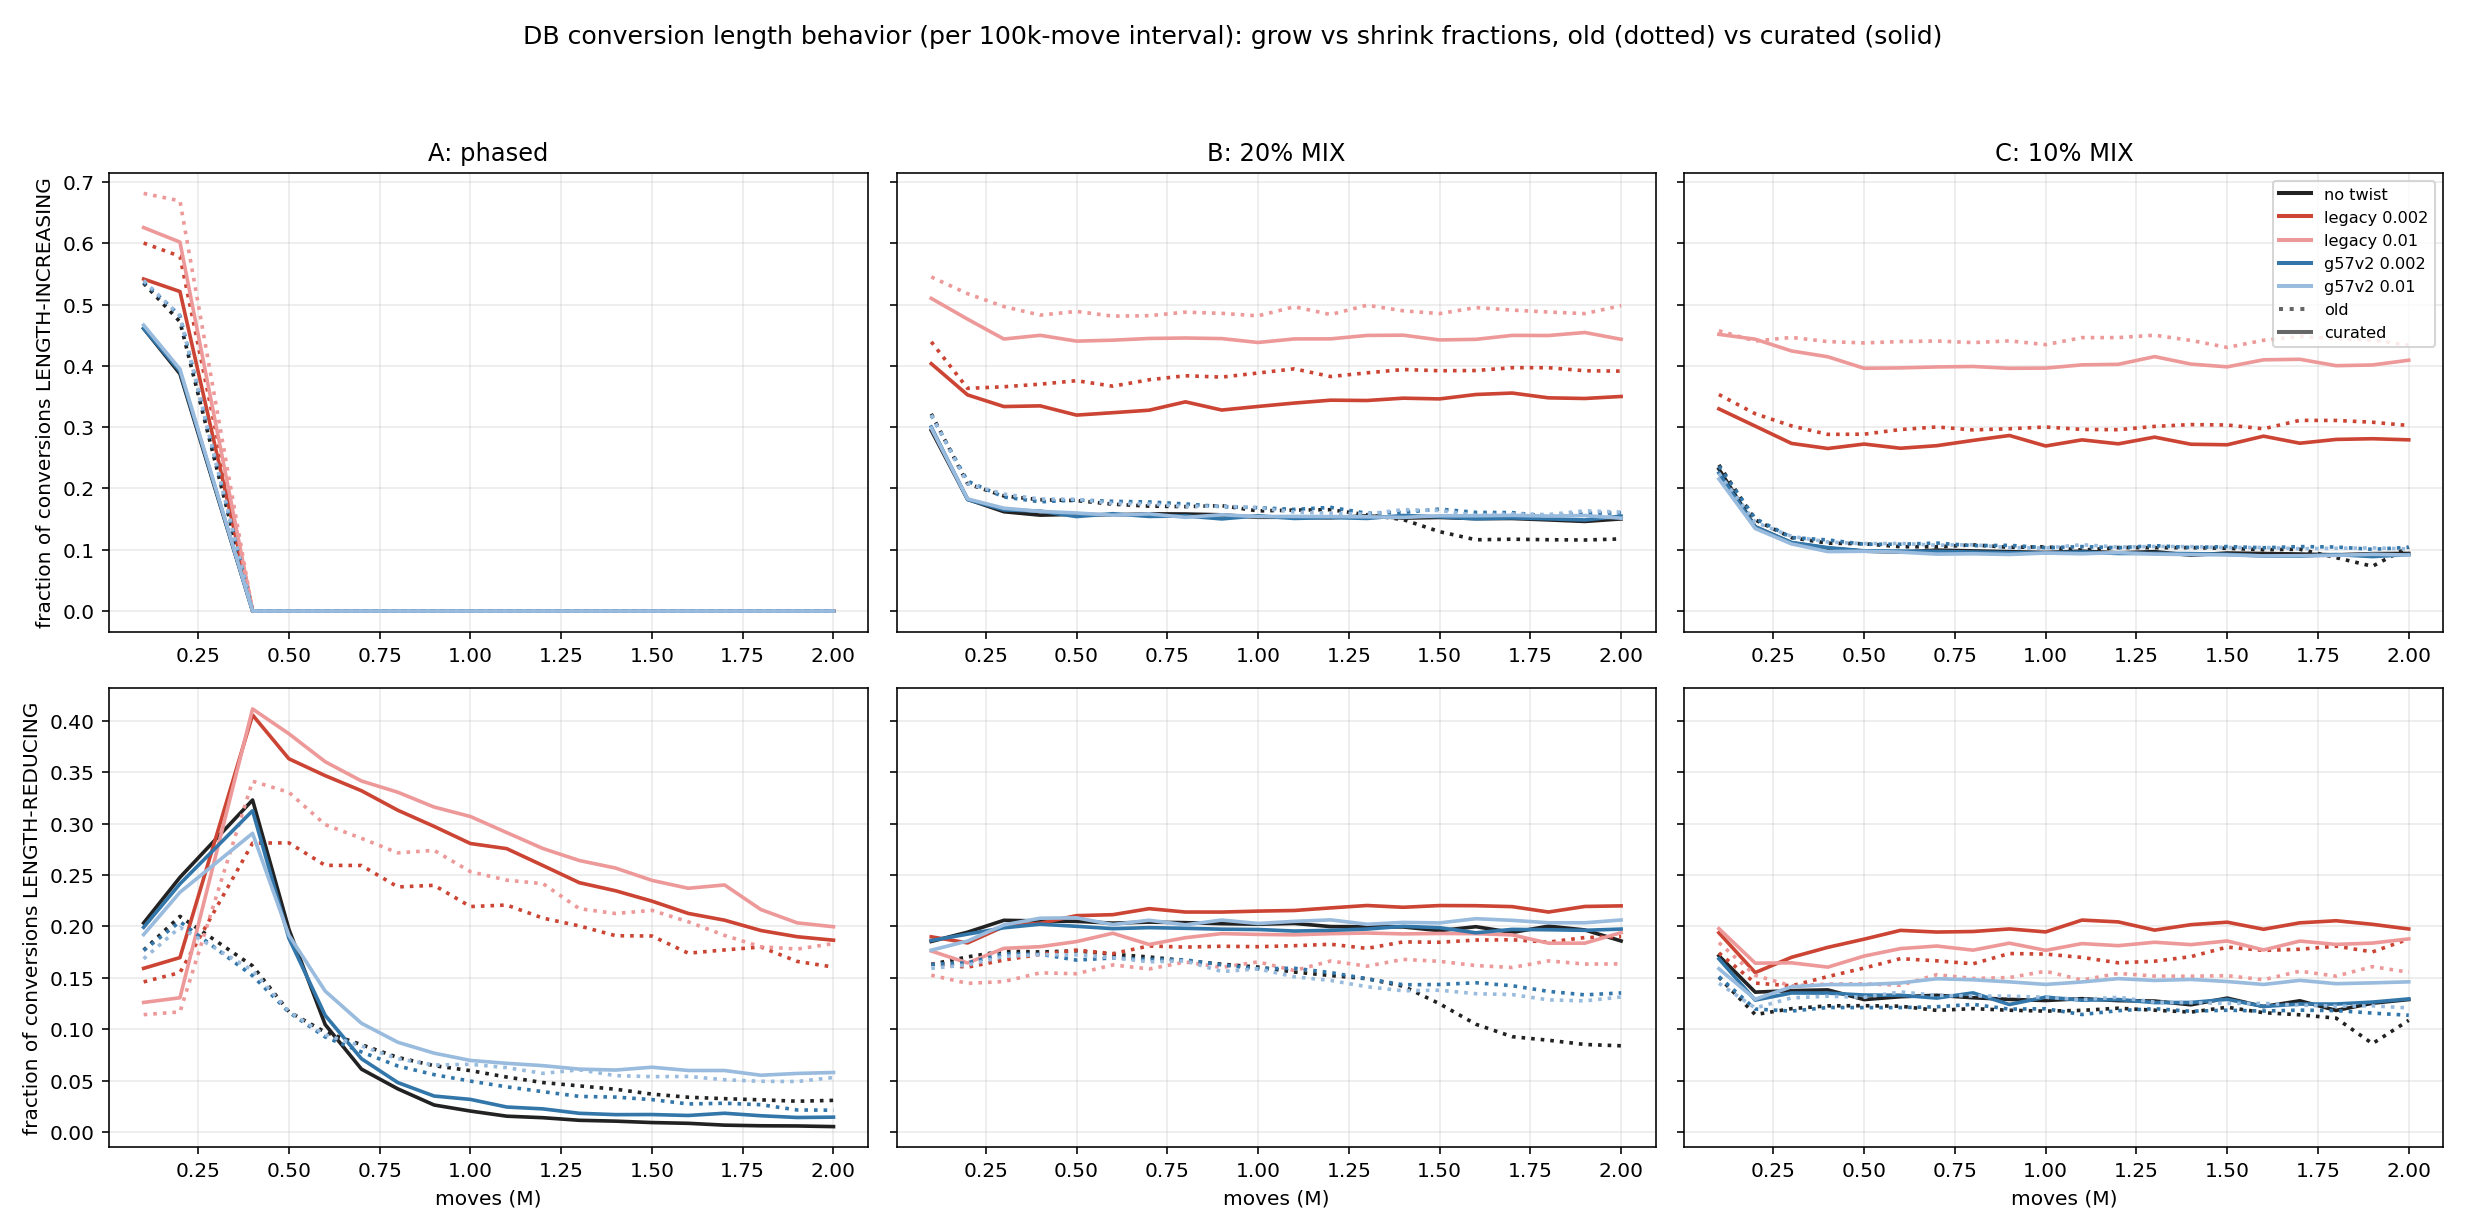
\includegraphics[width=\textwidth]{../reports/ancestry_20260728/abc_growshrink_20260730.png}
\caption{Grow/shrink conversion fractions, old (dotted) vs.\ new (solid).}
\end{figure}
\begin{figure}[h]\centering
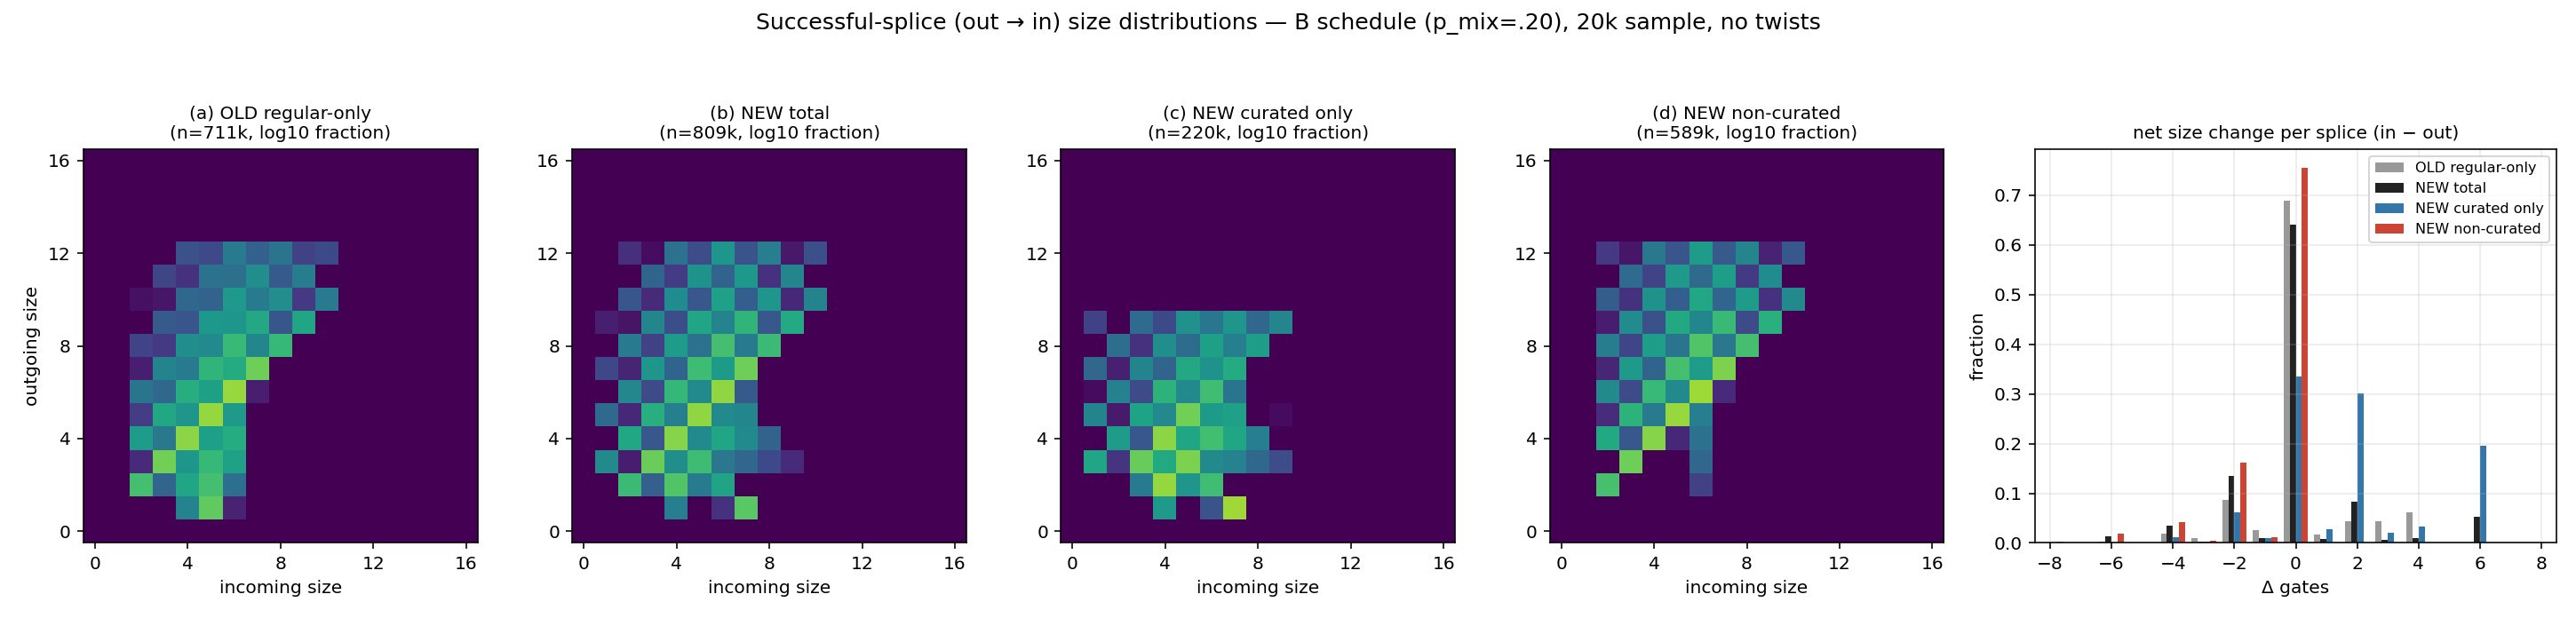
\includegraphics[width=\textwidth]{../reports/ancestry_20260728/splice_dist_abcd_20260731.png}
\caption{The four-way splice-size decomposition (a/b/c/d).}
\end{figure}

\end{document}
